\subsection{Main Processor Module State and Conclusion} \label{subsec:MCUConclusion}

The Main Processor Module integrates all essential functions to interface with the Sample Control module, calibrate the instrument, enable auto-ranging features, and conduct spectral analysis. It is fully capable of initiating the sampling process, retrieving samples, analyzing them via spectral analysis, and calculating the impedance of the DUT as described in Section \refq{sec:ImpedanceAnalysis}. However, the module's code remains incomplete at the time of this report, primarily due to its dependency on the development of the User Interface (UI).

The HMI uses a Nextion NX8048P070 Intelligent Series 7" touchscreen display development board \cite{NextionDisplay}. Although incomplete at the time of this report, the \textbf{work-in-progress} interface is shown in Figure \ref{fig:7_3_3_NextionHMI}.

\begin{figure}[H] \centering 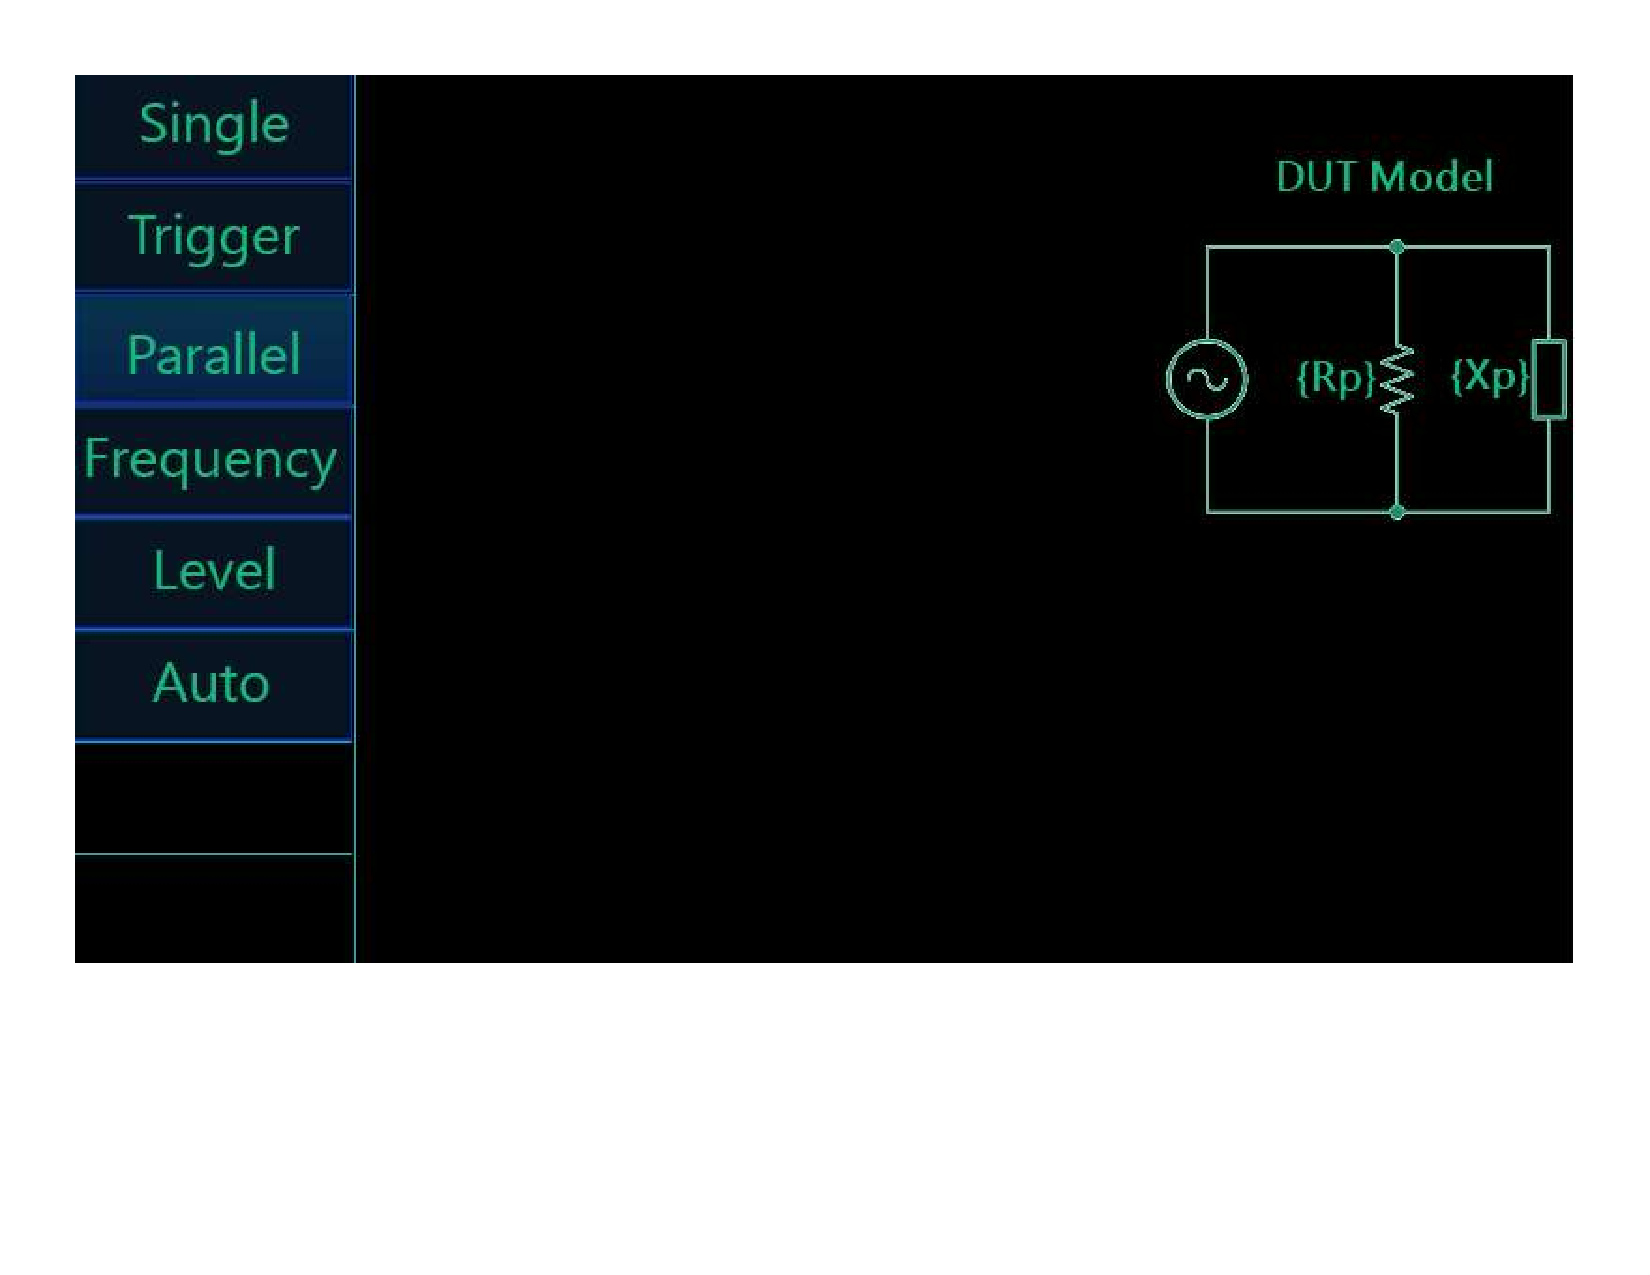
\includegraphics[clip, trim=0 150 0 0, width=0.65\textwidth]{Sections/7_SystemDesign/Figures/7_3_3_UIStatus.pdf} \caption{Current state of the HMI in the Nextion Editor. The UI includes buttons on the left side of the screen for setting various test parameters. The interface is currently in "single" measurement mode, indicated by the darkened "single" button. Pressing this button switches the interface to "sweep" mode, designed for generating plots as described earlier. The "parallel" model is selected, as shown by the corresponding highlighted button, which displays the parallel impedance model and measured parameters on the right side. The MCU detects whether the reactance is positive or negative and adjusts the Xp component to represent a capacitor or inductor accordingly. Final measurements of R, L, C, D, Q, and related parameters will be displayed in the center of the screen but are not yet implemented.} \label{fig:7_3_3_NextionHMI} \end{figure}

The Nextion platform simplifies integration using its proprietary display editor, which expedites the design process. The display communicates with the STM32 via UART, and basic data transfer has been successfully tested. However, a comprehensive data structure for display communication has not yet been implemented. One drawback of this platform is the time required to create graphical elements. Due to the absence of technical challenges in integrating this display, its development was assigned lower priority from the beginning of the project and remains incomplete.

Data from the impedance analyzer can be retrieved through a UART connection with the STM32, as shown in figure \refq{fig:7_3_3_CapMeasSerialPrint}.

\begin{figure}[H] \centering 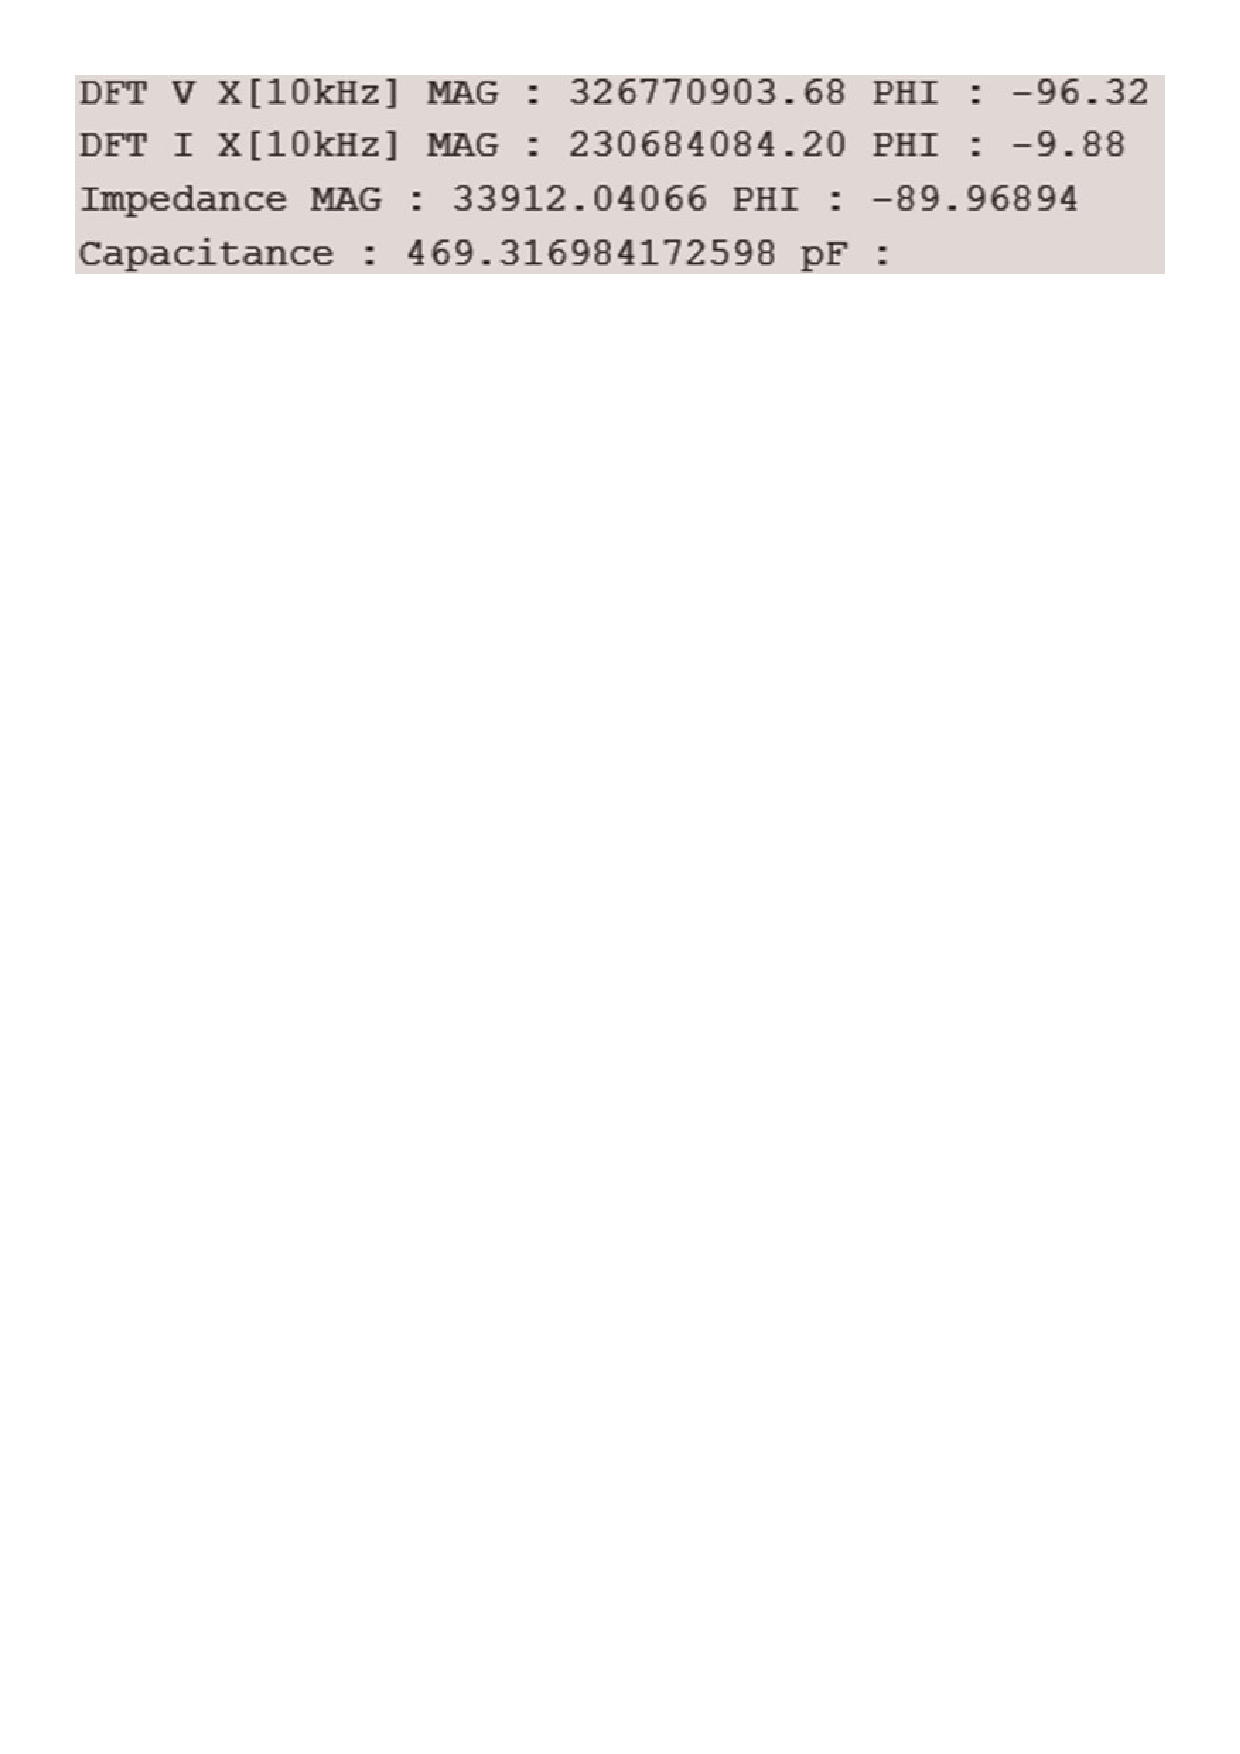
\includegraphics[clip, trim=0 700 0 0, width=0.65\textwidth]{Sections/7_SystemDesign/Figures/7_3_3_CapMeasuredSerialPrint.pdf} \caption{A DUT has been measured at \SIQ{10}{\kilo\hertz} by the impedance analyzer and the results are transmitted over a UART connection. Line 1-2 show the results from the DFT on the DUT voltage and currents. Line 3 shows the calculated impedance of the DUT in polar form and the magnitude and phase of the impedance is listed. Line 4 shows that the instrument has correctly identified the DUT as a capacitor with a value of about $470pF$. The DUT is a \SIQ{470}{\pico\farad} 1\% Mica capacitor.} \label{fig:7_3_3_CapMeasSerialPrint} \end{figure}

The instrument can take measurements of the DUT impedance as shown in figure \refq{fig:7_3_3_CapMeasSerialPrint} and display them to the user. Only the capacitance value of the DUT is shown, but it could also have listed the loss tangent, ESR or any other desired parameter as well.

In summary, the Main Processor Module includes all functionality required for the instrument to operate. However, the absence of finalized functions to display results to the user remains a limitation at this stage and a polished main() loop has not been developed.